\chapter{Evaluation and Results}

% \section{Curriculum Effectiveness}

% \section{Chatbot Performance and Usefulness}

% \section{Case Study}
%     \subsection{Results and Analysis}
%     The evaluation of the compressing the BART-Base model using low-rank approximation reveals the following insights:
    
%     \textbf{ROUGE scores:} The low-rank approximation technique achieve comparable ROUGE scores until rank \(r = 510\), after which the scores begin to decline. This indicates that the model's performance is preserved up to a certain rank, beyond which the approximation starts to impact the summarization quality.
%     \begin{figure}[htbp]
%         \centering
%         \begin{subfigure}[b]{0.45\textwidth}
%             \centering
%             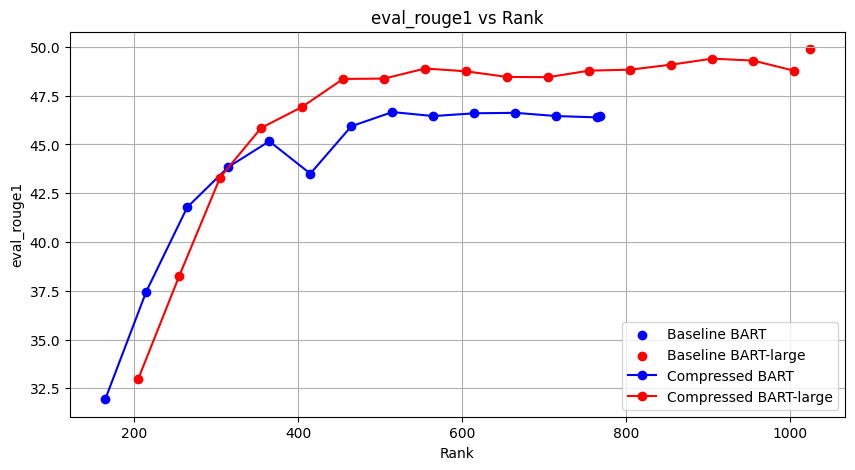
\includegraphics[width=\textwidth]{figs/05:05/Rouge1.png}
%             \caption{Rouge1 scores.}
%             \label{fig:sub1}
%         \end{subfigure}
%         \hfill
%         \begin{subfigure}[b]{0.45\textwidth}
%             \centering
%             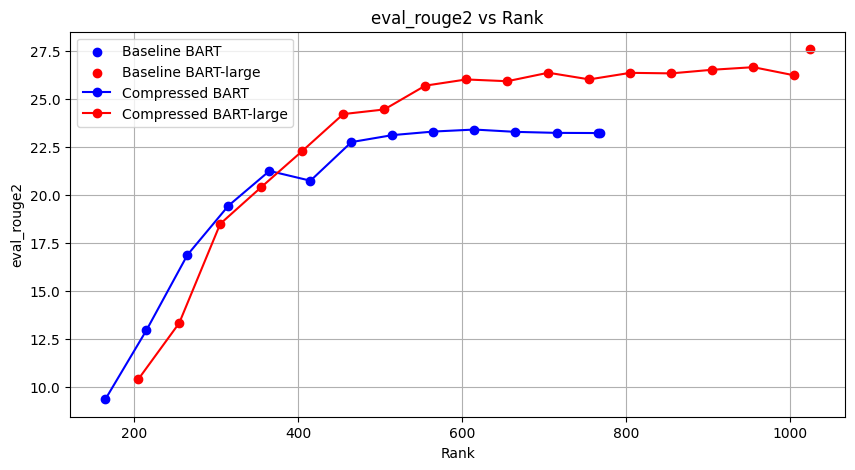
\includegraphics[width=\textwidth]{figs/05:05/Rouge2.png}
%             \caption{Rouge2 scores.}
%             \label{fig:sub2}
%         \end{subfigure}
%         \vskip\baselineskip
%         \begin{subfigure}[b]{0.45\textwidth}
%             \centering
%             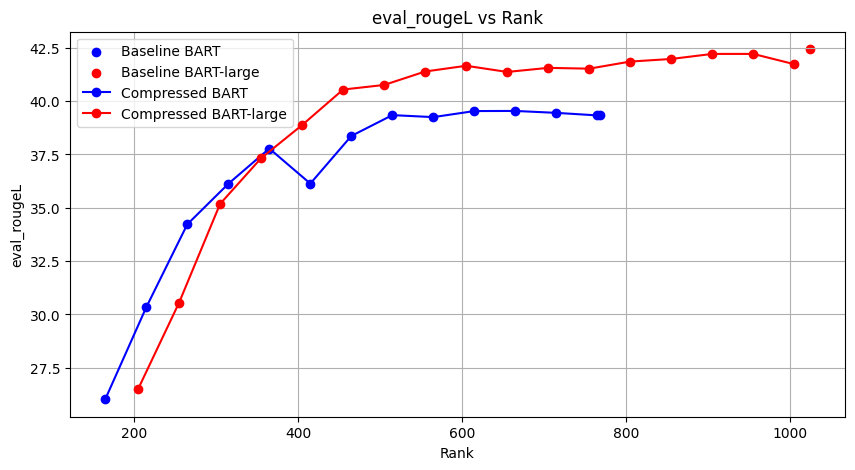
\includegraphics[width=\textwidth]{figs/05:05/RougeL.png}
%             \caption{RougeL scores.}
%             \label{fig:sub3}
%         \end{subfigure}
%         \hfill
%         \begin{subfigure}[b]{0.45\textwidth}
%             \centering
%             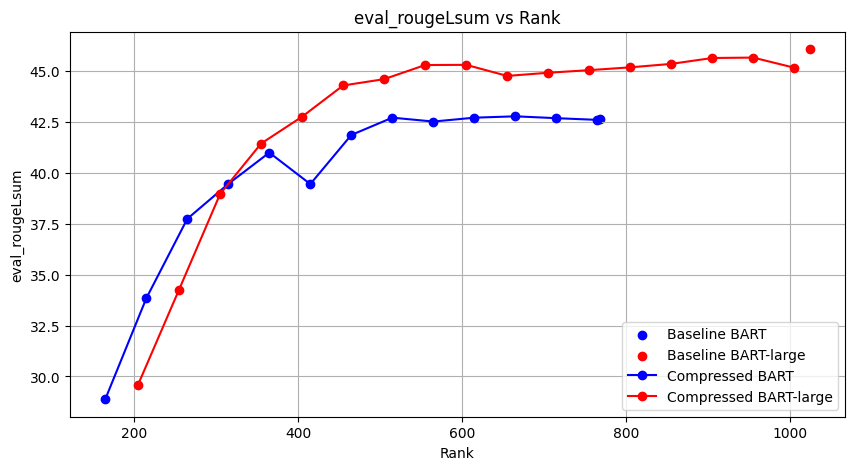
\includegraphics[width=\textwidth]{figs/05:05/RougeLSum.png}
%             \caption{RougeLsum scores.}
%             \label{fig:sub4}
%         \end{subfigure}
%         \caption{ROUGE scores for different ranks}
%         \label{fig:main}
%     \end{figure}
%     Recall in \ref{appropriate_rank} that we needed to low-rank approximate the self-attention matrices with at most rank \(r = 318\) to achieve a reduction in computational complexity and storage requirements.

    
%     \textbf{Computational Efficiency:}
%         \begin{figure}[H]
%             \centering
%             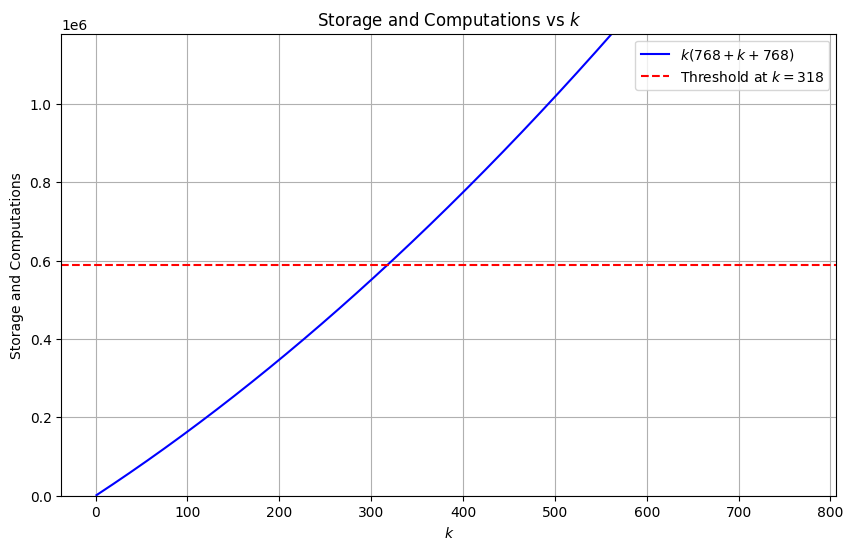
\includegraphics[width=0.7\textwidth]{figs/05:05/Efficiency.png}
%             \caption{Computational efficiency comparison}
%             \label{fig:ComputationalEfficiency}
%         \end{figure}


    \section{Case Study}
    \subsection{Results and Analysis}
    The evaluation of compressing the BART-base and BART-large model using low-rank approximation reveals the following insights:
    
    \textbf{ROUGE scores:} The low-rank approximation technique achieves comparable ROUGE scores until rank \(r = 510\), after which the scores begin to decline. This indicates that the model's performance is preserved up to a certain rank, beyond which the approximation starts to impact the summarization quality. The following figures illustrate the ROUGE scores for various ranks:
    
    \begin{figure}[H]
        \centering
        \begin{subfigure}[b]{0.45\textwidth}
            \centering
            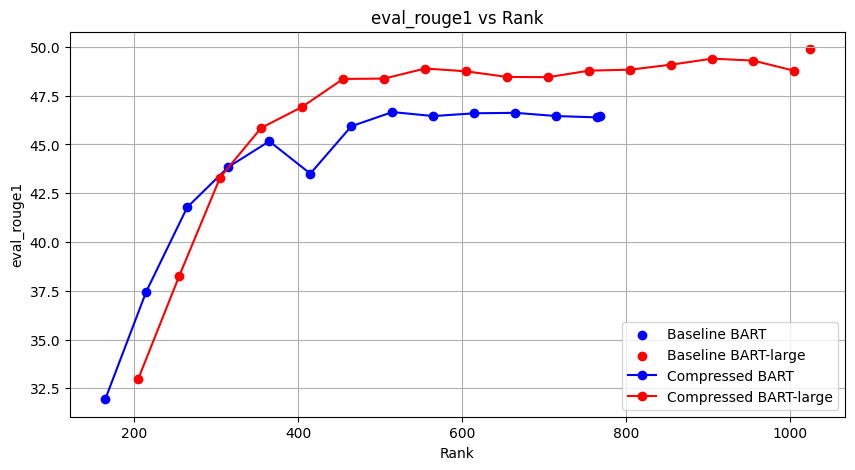
\includegraphics[width=\textwidth]{figs/05:05/Rouge1.png}
            \caption{ROUGE-1 scores.}
            \label{fig:sub1}
        \end{subfigure}
        \hfill
        \begin{subfigure}[b]{0.45\textwidth}
            \centering
            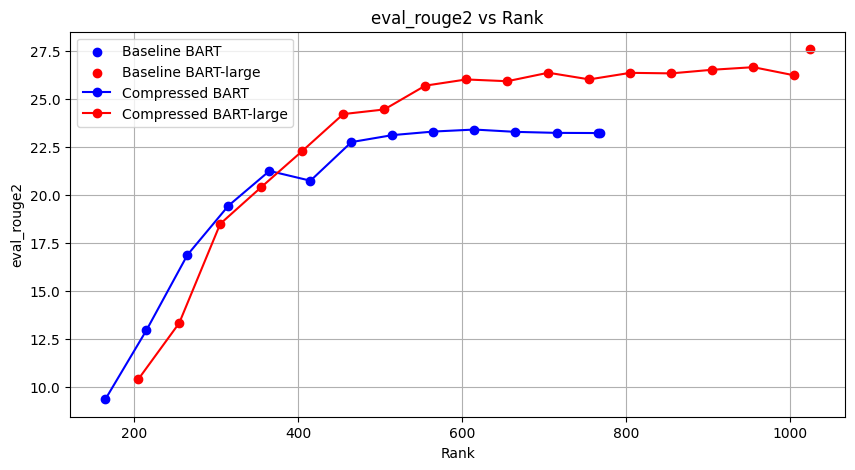
\includegraphics[width=\textwidth]{figs/05:05/Rouge2.png}
            \caption{ROUGE-2 scores.}
            \label{fig:sub2}
        \end{subfigure}
        \vskip\baselineskip
        \begin{subfigure}[b]{0.45\textwidth}
            \centering
            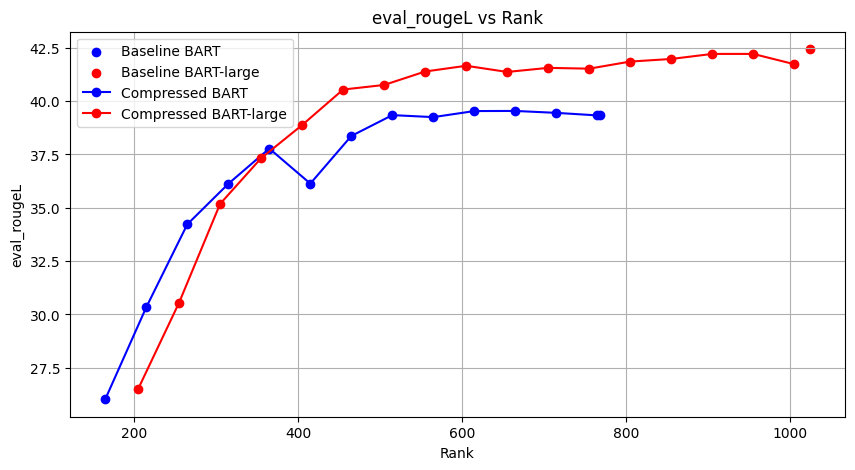
\includegraphics[width=\textwidth]{figs/05:05/RougeL.png}
            \caption{ROUGE-L scores.}
            \label{fig:sub3}
        \end{subfigure}
        \hfill
        \begin{subfigure}[b]{0.45\textwidth}
            \centering
            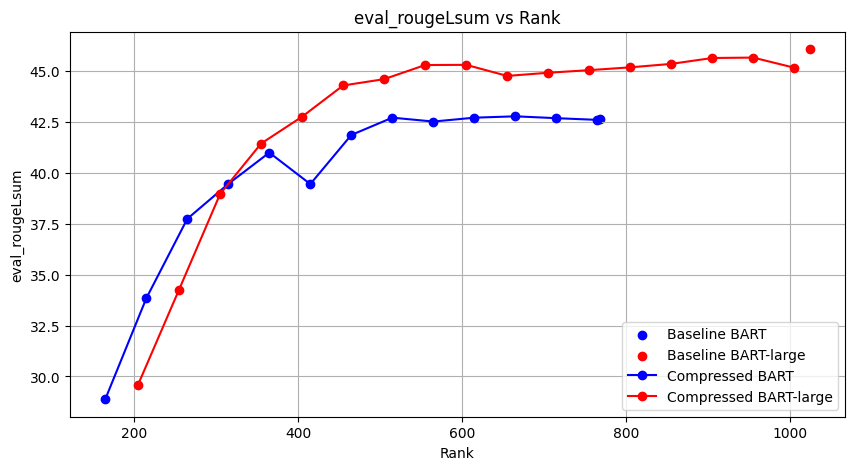
\includegraphics[width=\textwidth]{figs/05:05/RougeLSum.png}
            \caption{ROUGE-Lsum scores.}
            \label{fig:sub4}
        \end{subfigure}
        \caption{ROUGE scores for different ranks.}
        \label{fig:main}
    \end{figure}
    
    As depicted in Figure \ref{fig:main}, the ROUGE-1, ROUGE-2, ROUGE-L, and ROUGE-Lsum scores maintain a high level of performance up to a rank of \(r = 510\). However, it is important to note that for the BART-large model, there is a slight decline in performance even when the model is low-rank approximated at full rank. Beyond the rank of \(r = 510\), a noticeable degradation in scores is observed, indicating the limitations of the low-rank approximation in preserving the model's quality.

    \textbf{Cosine Similarity:}

    \textbf{Comparing Summaries:}
        
    \textbf{Computational Complexity and Storage Requirements:}
    Recall from Section \ref{appropriate_rank} that we needed to low-rank approximate the self-attention matrices with at most rank \(r = 318\) and rank \(r = 424\) for BART-base and BART-large respectively to achieve a significant reduction in computational complexity and storage requirements. However, the results show that the summarization quality declines significantly before this threshold.


    \subsection{Conclusion}
    The low-rank approximation of the BART-Base model does not present a viable approach to compressing large language models for summarization tasks. Although the technique can achieve significant reductions in computational complexity and storage requirements, the summarization quality declines significantly before reaching a practically useful rank. These findings highlight the limitations of low-rank approximations for preserving the performance of large language models in summarization tasks.
    
    In summary, while low-rank approximation effectively reduces the computational burden and storage requirements of the BART-Base model, the associated decline in summarization quality limits its practical applicability. This work underscores the need for alternative approaches to optimize and deploy large language models in resource-constrained environments without compromising performance.
    